
The result of our selection protocol is a benchmark with 200 stack traces called \emph{\crashpack}. 
For each stack trace, based on the information from the issue tracker and the Defects4J data, we collected: the \emph{Java project} in which the crash happened, the \emph{version} of the project where the crash happened and (when available) the \emph{fixed version}  or the fixing commit reference of the project; the \emph{buggy frame} (i.e., the frame in the stack trace targeting the method where the bug lays); and the \emph{Cyclomatic Complexity Number (CCN)} and the \emph{Non-Com\-men\-ting Sources Statements (NCSS)} of the project, presented in Figure \ref{fig:ccnncssperapp}. 
Due to the manual effort involved in filtering, verifying and cleaning up stack traces, issues, the collection of stack traces and binaries (including the project's dependencies binaries) took about 4.5 person-months in total.

\begin{figure}[t]
  \centering
  \subfloat[Average methods Cyclomatic Complexity Number (CCN)]{%
  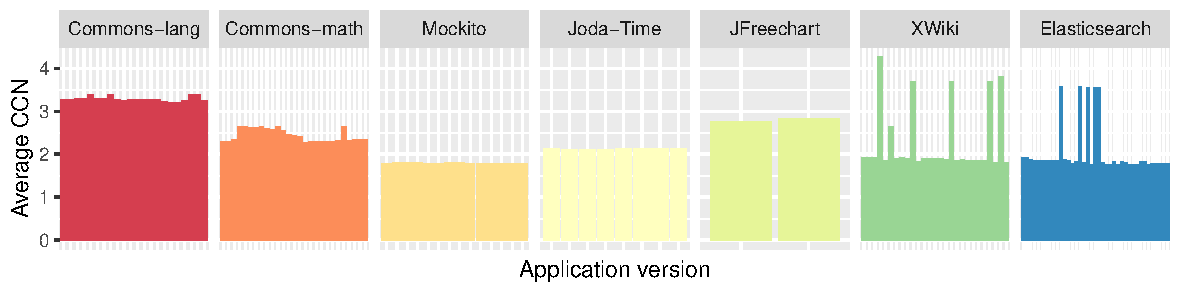
\includegraphics[width=0.98\textwidth]{papers/jcrashpack/benchmark-ccn-per-app-histogram}
  \label{fig:ccnperapp}
  }\\
  \subfloat[Thousands of Non-Com\-men\-ting Sources Statements (KNCSS)]{
%    	\includegraphics[width=0.80\textwidth]{benchmark-ncss-per-app-boxplot}
    	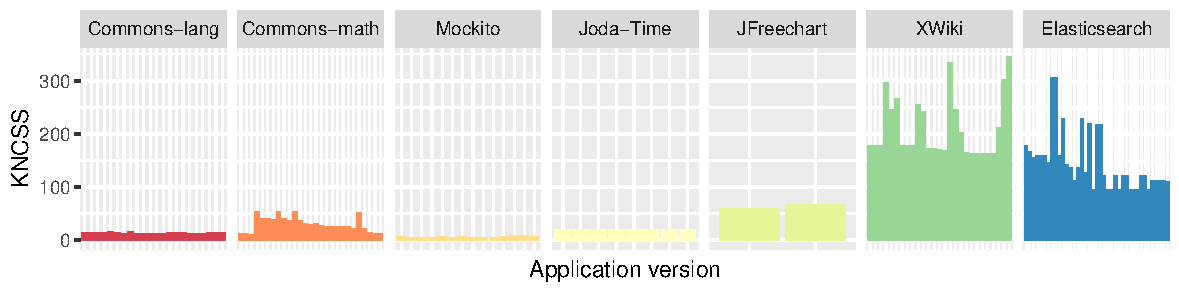
\includegraphics[width=0.98\textwidth]{papers/jcrashpack/benchmark-ncss-per-app-histogram}
    \label{fig:ncssperapp}
  }
  \caption{Complexity and size of the different projects}
  \label{fig:ccnncssperapp}
\end{figure}

Figure \ref{fig:ccnncssperapp} presents the average Cyclomatic Complexity Number (CCN) per method for each project and the Non-Com\-men\-ting Sources Statements (NCSS) per project, ordered by version number, to give an idea of the complexity of a project. Also, Table \ref{tab:benchmark:complexity} gives the number of versions and the average number of non-commenting source statement for each project in \crashpack.
As illustrated in the table and figure, \crashpack contains projects of diverse complexities (the CCN for the least complex project is 1.77, and for the most complex is 3.38) and sizes (the largest project has 177,840 statements, and the smallest one holds 6,060 statements on average), distributed among different versions.

\begin{table*}[t]
	\centering
	\caption{The number of versions and average number of statements ($\overline{NCSS}$) for each project.}
	\label{tab:benchmark:complexity}
	\begin{tabular}{ l | c r } \textbf{Applications} & \textbf{Number of versions} & \textbf{$\overline{NCSS}$}\\
\hline 
\textbf{ Commons-lang } & 22 & 13.38k \\
\textbf{ Commons-math }  & 27 & 29.98k \\
\textbf{ Mockito } & 14 & 6.06k \\
\textbf{ Joda-Time } & 8 & 19.41k \\
\textbf{ JFreechart } & 2 & 63.01k \\
\textbf{ XWiki } & 32 & 177.84k \\
\textbf{ Elasticsearch } & 46 & 124.36k \\
\textbf{ Total } & 151 & 62.01k \\
\end{tabular}
\end{table*}

\begin{table*}[t]
	\centering
	\caption{Number of stack traces (\textit{st}), total number of frames (\textit{fr}), and average number of frames ($\overline{fr}$) and standard deviation ($\sigma$) per stack trace for the different exceptions: NullPointerException (NPE), IllegalArgumentException (IAE), ArrayIndexOutOfBoundsException (AIOOBE), ClassCastException (CCE), StringIndexOutOfBoundsException (SIOOBE), IllegalStateException (ISE), and other exceptions types (Other). }
	\label{tab:benchmark}
%	\input{benchmark-exceptionsapps-table.tex}
    \begin{scriptsize}
	% NullPointerException (NPE), IllegalArgumentException (IAE), ArrayIndexOutOfBoundsException (AIOOBE), ClassCastException (CCE), StringIndexOutOfBoundsException (SIOOBE), IllegalStateException (ISE), Other (Other), 
\begin{tabular}{ l l | r r r r r r r | r } \textbf{Applications} & & \textbf{\rotatebox{90}{ NPE }} & \textbf{\rotatebox{90}{ IAE }} & \textbf{\rotatebox{90}{ AIOOBE }} & \textbf{\rotatebox{90}{ CCE }} & \textbf{\rotatebox{90}{ SIOOBE }} & \textbf{\rotatebox{90}{ ISE }} & \textbf{\rotatebox{90}{ Other }} & \textbf{ Total } \\ 
\hline 
\textbf{ Commons-lang } & \textit{st}  & 5.0 & 3.0 & 2.0 & 0.0  & 6.0 & 0.0  & 6.0 & 22.0\\ 
  & \textit{fr}  & 8.0 & 3.0 & 12.0 & 0.0 & 10.0 & 0.0 & 12.0 & 45.0\\ 
  & $\overline{fr}$  & 1.6 & 1.0 & 6.0 &   & 1.7 &   & 2.0 & 2.0\\ 
 & $\sigma$  & 0.9 & 0.0 & 5.7 &   & 1.0 &   & 1.5 & 2.1\\ 
\hline 
\textbf{ Commons-math } & \textit{st}  & 3.0 & 3.0 & 4.0 & 2.0 & 1.0 & 0.0  & 14.0 & 27.0\\ 
  & \textit{fr}  & 8.0 & 7.0 & 9.0 & 11.0 & 1.0 & 0.0 & 70.0 & 106.0\\ 
  & $\overline{fr}$  & 2.7 & 2.3 & 2.2 & 5.5 & 1.0 &   & 5.0 & 3.9\\ 
 & $\sigma$  & 0.6 & 1.5 & 2.5 & 6.4 & NA &   & 3.0 & 3.0\\ 
\hline 
\textbf{ Mockito } & \textit{st}  & 2.0 & 0.0  & 2.0 & 2.0 & 0.0  & 0.0  & 8.0 & 14.0\\ 
  & \textit{fr}  & 3.0 & 0.0 & 12.0 & 2.0 & 0.0 & 0.0 & 48.0 & 65.0\\ 
  & $\overline{fr}$  & 1.5 &   & 6.0 & 1.0 &   &   & 6.0 & 4.6\\ 
 & $\sigma$  & 0.7 &   & 7.1 & 0.0 &   &   & 3.8 & 4.1\\ 
\hline 
\textbf{ Joda-Time } & \textit{st}  & 0.0  & 3.0 & 0.0  & 0.0  & 0.0  & 0.0  & 5.0 & 8.0\\ 
  & \textit{fr}  & 0.0 & 5.0 & 0.0 & 0.0 & 0.0 & 0.0 & 26.0 & 31.0\\ 
  & $\overline{fr}$  &   & 1.7 &   &   &   &   & 5.2 & 3.9\\ 
 & $\sigma$  &   & 0.6 &   &   &   &   & 1.5 & 2.2\\ 
\hline 
\textbf{ JFreechart } & \textit{st}  & 1.0 & 1.0 & 0.0  & 0.0  & 0.0  & 0.0  & 0.0  & 2.0\\ 
  & \textit{fr}  & 6.0 & 6.0 & 0.0 & 0.0 & 0.0 & 0.0 & 0.0 & 12.0\\ 
  & $\overline{fr}$  & 6.0 & 6.0 &   &   &   &   &   & 6.0\\ 
 & $\sigma$  & NA & NA &   &   &   &   &   & 0.0\\ 
\hline 
\textbf{ XWiki } & \textit{st}  & 20.0 & 4.0 & 0.0  & 6.0 & 1.0 & 0.0  & 20.0 & 51.0\\ 
  & \textit{fr}  & 535.0 & 39.0 & 0.0 & 131.0 & 8.0 & 0.0 & 687.0 & 1400.0\\ 
  & $\overline{fr}$  & 26.8 & 9.8 &   & 21.8 & 8.0 &   & 34.4 & 27.5\\ 
 & $\sigma$  & 33.3 & 3.7 &   & 22.2 & NA &   & 47.0 & 37.0\\ 
\hline 
\textbf{ Elasticsearch } & \textit{st}  & 18.0 & 10.0 & 6.0 & 0.0  & 1.0 & 7.0 & 34.0 & 76.0\\ 
  & \textit{fr}  & 222.0 & 152.0 & 102.0 & 0.0 & 15.0 & 135.0 & 717.0 & 1343.0\\ 
  & $\overline{fr}$  & 12.3 & 15.2 & 17.0 &   & 15.0 & 19.3 & 21.1 & 17.7\\ 
 & $\sigma$  & 9.8 & 9.2 & 18.0 &   & NA & 11.9 & 13.4 & 12.5\\ 
\hline 
 \textbf{Total}  & \textit{st}  & 49.0 & 24.0 & 14.0 & 10.0 & 9.0 & 7.0 & 87.0 & 200.0\\ 
  & \textit{fr}  & 782.0 & 212.0 & 135.0 & 144.0 & 34.0 & 135.0 & 1560.0 & 3002.0\\ 
  & $\overline{fr}$  & 16.0 & 8.8 & 9.6 & 14.4 & 3.8 & 19.3 & 17.9 & 15.0\\ 
 & $\sigma$  & 23.9 & 8.5 & 13.3 & 19.3 & 4.8 & 11.9 & 26.3 & 22.3\\ 
\end{tabular} 
    \end{scriptsize}
\end{table*}

Table \ref{tab:benchmark} shows the distribution of stack traces per exception type for the six most 
common ones, the \textit{Other} category denoting remaining exception types. According to this table, the included stack traces in \crashpack covers different types of the exceptions. Also, they are varied in the size (number of frames): the smallest stack traces have one frame and the largest, a user-defined exception in \textit{Other}, has 175 frames.

\crashpack is extensible and publicly available on GitHub.\footnote{At \url{https://github.com/STAMP-project/JCrashPack}} We provide guidelines to add new crashes to the benchmark and make a pull request to include them in \crashpack master branch.
%
The detailed numbers for each stack trace and its project are available on the \crashpack website.

